\begin{center}
    {\Huge \textbf{Доказательства}}
\end{center}
\addcontentsline{toc}{section}{Определения}
\section{3-й модуль}

\subsection{Дайте определение кольца. Приведите пример.}

\begin{definition}
    $K \neq \varnothing$ --- множество с двумя бинарными операциями: $+$ и $\cdot$, то есть
    \[
        1)\ (K, +) \text{ --- абелева группа}
    \]
    \[
        2)\ (K, \cdot) \text{ --- полугруппа}
    \]
    \[
        3)\ \text{Дистрибутивность: } (a + b)c = ac + bc,\ c(a + b) = ca + cb
    \]
\end{definition}
\begin{example}
    \[
        (\mathbb{Z}, +, \cdot) \text{ --- кольцо}
    \]
\end{example}


\subsection{Что такое коммутативное кольцо? Приведите примеры коммутативного и некоммутативного колец.}

\begin{definition}
    $\forall x, y \in K\ xy = yx$, то кольцо $(K, +, \cdot)$ называется коммутативным
\end{definition}

\begin{example}
    \[
        (\mathbb{Z}, +, \cdot) \text{ --- коммутативное кольцо}
    \]
\end{example}

\begin{example}
    \[
        (M_n(\mathbb{R}), +, \cdot) \text{ --- некоммутативное кольцо}
    \]
\end{example}


\subsection{Дайте определение делителей нуля. Приведите пример.}

\begin{definition}
    Если $ab = 0$ при $a \neq 0$ и $b \neq 0$ в кольце $K$, то $a$ называется левым, $b$ --- правым делителем нуля.
\end{definition}
\begin{example}
    В кольце $\mathbb{Z}_6$:
    \[
        2 \cdot 3 = 0,\quad 2 \neq 0,\quad 3 \neq 0
    \]
    значит $2$ и $3$ --- делители нуля.
\end{example}


\subsection{Дайте определение целостного кольца. Приведите пример.}

\begin{definition}
    Целостное кольцо --- коммутативное кольцо с $1 \neq 0$, не имеющее делителей нуля.
\end{definition}
\begin{example}
    \[
        (\mathbb{Z}, +, \cdot) \text{ --- целостное кольцо}
    \]
\end{example}


\subsection{Дайте определение поля. Приведите три примера.}

\begin{definition}
    Поле $P$ --- это коммутативное кольцо с единицей $(1 \neq 0)$, в котором каждый элемент $(\neq 0)$ обратим.
\end{definition}
\begin{example}
    \[
        (\mathbb{Q}, +, \cdot) \text{ --- поле}
    \]
\end{example}

\begin{example}
    \[
        (\mathbb{R}, +, \cdot) \text{ --- поле}
    \]
\end{example}

\begin{example}
    \[
        (\mathbb{C}, +, \cdot) \text{ --- поле}
    \]
\end{example}


\subsection{Дайте определение подполя. Привести пример пары: поле и его подполе.}

\begin{definition}
    Подполе --- подмножество поля, которое само является полем относительно тех же операций.
\end{definition}

\begin{example}
    \[
        \mathbb{Q} \subset \mathbb{R}
    \]
\end{example}


\subsection{Дайте определение характеристики поля. Привести примеры: поля конечной положительной характеристики и поля нулевой характеристики.}

\begin{definition}
    $P$ --- поле. Характеристикой поля называется такое наименьшее число $q \in \mathbb{N}$:
    \[
        \underbrace{1 + 1 + \ldots + 1}_{q} = 0.
    \]
    Если такого $q$ нет, то $\operatorname{char} P = 0$.
\end{definition}

\begin{example}
    \[
        \operatorname{char} \mathbb{R} = 0
    \]
\end{example}

\begin{example}
    \[
        \operatorname{char} \mathbb{Z}_p = p
    \]
\end{example}


\subsection{Сформулируйте утверждение о том, каким будет простое подполе в зависимости от характеристики.}

\begin{theorem}
    $P$ --- поле, $P_0$ --- его простое подполе. Тогда:
    \[
        1)\ \operatorname{char} P = p > 0,\ \text{то } P_0 \cong \mathbb{Z}_p
    \]
    \[
        2)\ \operatorname{char} P = 0,\ \text{то } P_0 \cong \mathbb{Q}
    \]
\end{theorem}


\subsection{Дайте определение идеала.}

\begin{definition}
    Подмножество $I$ кольца $K$ называется идеалом, если оно:
    \[
        1)\ \text{является подгруппой } (K, +) \text{ по сложению}
    \]
    \[
        2)\ \forall a \in I\ \forall r \in K\quad ra \in I \text{ и } ar \in I
    \]
\end{definition}


\subsection{Сформулируйте определение гомоморфизма колец. Приведите пример.}

\begin{definition}
    $\varphi: K_1 \to K_2$ --- гомоморфизм колец, если $\forall a, b \in K_1$:
    \[
        1)\ \varphi(a + b) = \varphi(a) \oplus \varphi(b)
    \]
    \[
        2)\ \varphi(a \cdot b) = \varphi(a) \times \varphi(b)
    \]
\end{definition}
\begin{example}
    Рассмотрим отображение
    \[
        \varphi: \mathbb{Z} \to \mathbb{Z}_n,\quad \varphi(a) = \overline{a}
    \]
    Тогда $\varphi$ --- гомоморфизм колец, так как
    \[
        \varphi(a + b) = \overline{a + b} = \overline{a} + \overline{b}
    \]
    \[
        \varphi(ab) = \overline{ab} = \overline{a}\cdot \overline{b}
    \]
\end{example}


\subsection{Сформулируйте теорему о гомоморфизме колец. Приведите пример.}

\begin{theorem}
    Пусть $K_1, K_2$ --- два кольца, $\varphi: K_1 \to K_2$ --- гомоморфизм. Тогда
    \[
        K_1 / \operatorname{Ker}\varphi \cong \operatorname{Im}\varphi
    \]
\end{theorem}

\begin{example}
    \[
        \mathbb{Z}/n\mathbb{Z} \cong \mathbb{Z}_n,\quad \varphi: \mathbb{Z} \to \mathbb{Z}_n
    \]
\end{example}


\subsection{Сформулируйте критерий того, что кольцо вычетов по модулю n является полем.}

\begin{theorem}
    \[
        \mathbb{Z}_p \text{ является полем } \Longleftrightarrow p \text{ --- простое}
    \]
\end{theorem}


\subsection{Сформулируйте теорему о том, когда факторкольцо кольца многочленов над полем само является полем.}

\begin{theorem}
    $P$ --- поле, $f(x) \in P[x]$.
    \[
        P[x] / \langle f(x) \rangle \text{ --- поле } \Longleftrightarrow f(x) \text{ неприводим над } P.
    \]
\end{theorem}


\subsection{Дайте определение алгебраического элемента над полем.}

\begin{definition}
    Элемент $x \in P$ называется алгебраическим элементом над полем $F \subset P$, если $\exists f(x) \neq 0$,
    \[
        f(x) \in F[x]:\quad f(a) = 0
    \]
\end{definition}


\subsection{Сформулируйте утверждение о том, что любое конечное поле может быть реализовано как факторкольцо кольца многочленов по некоторому идеалу.}

\begin{theorem}
    Любое конечное поле $F_q$, $q = p^n$, $p$ --- простое, можно реализовать в виде
    \[
        \mathbb{Z}_p[x] / \langle h(x) \rangle,
    \]
    где $h(x)$ --- неприводимый над $\mathbb{Z}_p[x]$.
\end{theorem}


\subsection{Сформулируйте утверждение о том, сколько элементов может быть в конечном поле.}

\begin{theorem}
    В конечном поле обязательно $p^n$ элементов, где $p$ --- простое, $n \in \mathbb{N}$.
\end{theorem}


\subsection{Дайте определение линейного (векторного) пространства.}

\begin{definition}
    Поле $F$, $V$ --- произвольное множество, на котором задано 2 операции: сложение и умножение на число, т.е. элемент из $F$. Это означает:
    \[
        \forall x, y \in V\quad \exists x + y \in V
    \]
    и
    \[
        \forall \lambda \in F\quad \exists \lambda x \in V.
    \]
    Множество $V$ называется линейным пространством, если выполнены 8 свойств:
    \[
        \forall x, y, z \in V,\quad \forall \lambda, \eta \in F:
    \]
    \[
        1)\ (x + y) + z = x + (y + z) \text{ --- ассоциативность сложения}
    \]
    \[
        2)\ \text{Найдётся нейтральный элемент по сложению: } \exists 0 \in V:\ \forall x \in V\quad x + 0 = 0 + x = x
    \]
    \[
        3)\ \exists \text{ противоположный по сложению: } \forall x \in V\ \exists (-x) \in V:\ x + (-x) = 0
    \]
    \[
        4)\ x + y = y + x
    \]
    \[
        5)\ \forall x \in V:\ 1 \cdot x = x,\ \text{нейтральный } 1 \in F
    \]
    \[
        6)\ \text{Ассоциативность умножения на число: } \lambda(\eta x) = (\lambda \eta)x
    \]
    \[
        7)\ \text{Дистрибутивность относительно сложения векторов: } \lambda(x + y) = \lambda x + \lambda y
    \]
    \[
        8)\ \text{Дистрибутивность относительно сложения чисел: } (\lambda + \eta)x = \lambda x + \eta x
    \]
\end{definition}


\subsection{Дайте определение базиса линейного (векторного) пространства.}

\begin{definition}
    Базисом линейного пространства $V$ называется упорядоченный набор векторов $b_1, \ldots, b_n$, т.ч.:
    \[
        1)\ b_1, \ldots, b_n \text{ --- л.н.з.}
    \]
    \[
        2)\ \text{любой вектор } v \in V \text{ представляется л.к. векторов } b_1, \ldots, b_n,
    \]
    то есть
    \[
        \forall x \in V\quad x = x_1 b_1 + \ldots + x_n b_n.
    \]
    При этом $x_1, \ldots, x_n$ называется координатами вектора $x$ в базисе $b_1, \ldots, b_n$.
\end{definition}


\subsection{Что такое размерность пространства?}

\begin{definition}
    Размерность пространства $V$ --- max число л.н.з. векторов в данном линейном простр. $V$.
\end{definition}

\begin{remark}[Обозначение]
    \[
        \dim V
    \]
\end{remark}


\subsection{Дайте определение матрицы перехода от старого базиса линейного пространства к новому.}

\begin{definition}
    Матрицей перехода от базиса $A$ к базису $B$ наз-ся м-ца:
    \[
        T_{A \to B} =
        \begin{pmatrix}
            t_{11} & \ldots & t_{1n} \\
            \ldots & \ldots & \ldots \\
            t_{n1} & \ldots & t_{nn}
        \end{pmatrix}
    \]
    \[
        (b_1, \ldots, b_n)_{1 \times n} = (a_1, \ldots, a_n) \cdot T_{A \to B}
    \]
    \[
        b = a \cdot T_{A \to B}
    \]
\end{definition}

\begin{remark}
    \[
        B = (b_1, \ldots, b_n),\quad A = (a_1, \ldots, a_n)
    \]
\end{remark}


\subsection{Выпишите формулу для описания изменения координат вектора при изменении базиса.}

\begin{definition}
    Ф-ла для описания изменения координат вектора при изменении базиса.
    
    \[
        \exists x \in L,\quad A, B \text{ --- базисы в } L
    \]
    \[
        x^a = (x_1^a, \ldots, x_n^a)^T
    \]
    --- столбец координат вектора $x$ в $A$.
    \[
        x^b = (x_1^b, \ldots, x_n^b)^T
    \]
    --- столбец координат вектора $x$ в $B$.
    
    Тогда
    \[
        x^b = T^{-1}_{A \to B} \cdot x^a
    \]
    \[
        x' = T^{-1}x
    \]
\end{definition}


\subsection{Дайте определение подпространства в линейном пространстве. Приведите 3 примера.}

\begin{definition}
    Подмножество $W$ векторного пространства $V$ называется подпространством, если оно само является пространством относительно операций в $V$.
\end{definition}
\begin{example}
    \[
        \{0\} \text{ --- подпространство в } V
    \]
\end{example}

\begin{example}
    \[
        V \text{ --- подпространство в } V
    \]
\end{example}

\begin{example}
    \[
        W = \{(x, y, 0)\ |\ x, y \in \mathbb{R}\}
        \text{ --- подпространство в } \mathbb{R}^3
    \]
\end{example}


\subsection{Дайте определения линейной оболочки конечного набора векторов и ранга системы векторов.}

\begin{definition}
    Множество
    \[
        L(a_1, \ldots, a_k) =
        \left\{
            \lambda_1 a_1 + \ldots + \lambda_k a_k\ |\ \lambda_i \in F
        \right\}
    \]
    --- множество всех л.к. векторов $a_1, \ldots, a_k$ называется линейной оболочкой набора $a_1, \ldots, a_k$.
\end{definition}

\begin{definition}
    Рангом системы векторов $a_1, \ldots, a_k$ в л.п. называется размерность их линейной оболочки:
    \[
        Rg(a_1, \ldots, a_k) = \dim(L(a_1, \ldots, a_k))
    \]
\end{definition}


\subsection{Дайте определения суммы и прямой суммы подпространств.}

\begin{definition}
    Множество
    \[
        H_1 + H_2 =
        \{x_1 + x_2\ |\ x_1 \in H_1,\ x_2 \in H_2\}
    \]
    называется суммой подпространств $H_1$ и $H_2$.
\end{definition}

\begin{definition}
    Сумма подпространств $H_1 + H_2$ называется прямой и обозначается
    \[
        H_1 \oplus H_2,
    \]
    где
    \[
        H_1 \cap H_2 = \{0\}.
    \]
\end{definition}


\subsection{Сформулируйте утверждение о связи размерности суммы и пересечения подпространств.}

\begin{theorem}
    $\exists H_1, H_2$ --- подпространства в $L$. Тогда
    \[
        \dim(H_1 + H_2) =
        \dim(H_1) + \dim(H_2) - \dim(H_1 \cap H_2)
    \]
\end{theorem}

\newpage





\section{4-й модуль}

\subsection{Дайте определения билинейной формы и матрицы билинейной формы.}

\begin{definition}
    $\exists V$ --- линейное пространство над $\mathbb{R}$.
    
    Функцию
    \[
        b: V \times V \to \mathbb{R}
    \]
    называют билинейной формой, если $\forall \alpha, \beta \in \mathbb{R}$:
    \[
        b(\alpha x + \beta y, z) = \alpha \cdot  b(x, z) + \beta \cdot b(y, z)
    \]
    \[
        b(x, \alpha y + \beta z) = \alpha \cdot (x, y)   + \beta \cdot b(x, z)
    \]
\end{definition}

\begin{definition}
    Матрицей билинейной формы:
    \[
        B_e = (b(e_i, e_j)),\quad i = \overline{1, n},\ j = \overline{1, n}
    \]
    называется матрицей билинейной формы в базисе $e$.
\end{definition}


\subsection{Дайте определение квадратичной формы и матрицы квадратичной формы.}

\begin{definition}
    Квадратичной формой: однородный многочлен от $n$ переменных, то есть:
    \[
        Q(x) = \sum_{i = 1}^{n} a_{ii}x_i^2 + 2\sum_{1 \leq i < j \leq n} a_{ij}x_i x_j,\quad a_{ij} \in \mathbb{R}
    \]
\end{definition}

\begin{definition}
    Матрица квадратичной формы.
\end{definition}


\subsection{Дайте определения положительной и отрицательной определенности квадратичной формы. Приведите примеры.}

\begin{definition}
    Квадратичная форма $Q(x)$ называется положительно определенной, если
    \[
        \forall x \neq 0\quad Q(x) > 0.
    \]
\end{definition}

\begin{example}
    \[
        Q(x) = x_1^2 + x_2^2
    \]
    положительно определена, так как
    \[
        \forall x \neq 0\quad Q(x) > 0.
    \]
\end{example}

\begin{definition}
    Квадратичная форма $Q(x)$ называется отрицательно определенной, если
    \[
        \forall x \neq 0\quad Q(x) < 0.
    \]
\end{definition}
\begin{example}
    \[
        Q(x) = -x_1^2 - x_2^2
    \]
    отрицательно определена, так как
    \[
        \forall x \neq 0\quad Q(x) < 0.
    \]
\end{example}

\subsection{Какую квадратичную форму называют знакопеременной? Приведите пример.}

\begin{definition}
    Квадратичная форма $Q(x)$ называется знакопеременной, если
    \[
        \exists x, y \in V\quad Q(x) < 0 < Q(y).
    \]
\end{definition}

\begin{example}
    \[
        Q(x) = x_1^2 - x_3^2
    \]
    \[
        y =
        \begin{pmatrix}
            1 \\
            0 \\
            0
        \end{pmatrix},
        \quad
        x =
        \begin{pmatrix}
            0 \\
            0 \\
            1
        \end{pmatrix}
    \]
\end{example}


\subsection{Дайте определения канонического и нормального вида квадратичной формы.}

\begin{definition}
    Квадратичную форму
    \[
        Q(x) = \alpha_1 x_1^2 + \ldots + \alpha_n x_n^2,\quad \alpha_i \in \mathbb{R},\ i = \overline{1, n}
    \]
    т.е. не имеющую попарных произведений $x_i x_j$, называют квадратичной формой канонического вида.
    
    Если $\alpha_i \in \{\pm 1, 0\}$, то канонический вид называют нормальным.
\end{definition}


\subsection{Как меняется матрица билинейной формы при замене базиса?}

\begin{theorem}
    При замене базиса матрица билинейной формы преобразуется по формуле:
    \[
        A' = C^TAC,
    \]
    где $C_{A \to A'}$, $A, A'$ --- конгруэтные матрицы.
\end{theorem}


\subsection{Как меняется матрица квадратичной формы при замене базиса?}
 
\begin{theorem}
    При переходе от базиса $E \to E'$ матрица квадратичной формы:
    \[
        A' = C^TAC,
    \]
    где $A'$ --- матрица квадратичной формы в базисе $E'$.
\end{theorem}


\subsection{Сформулируйте критерий Сильвестра и его следствие.}

\begin{theorem}[Критерий Сильвестра]
    Квадратичная форма $Q(x)$ от $n$ переменных
    \[
        x = (x_1, \ldots, x_n)^T
    \]
    положит. определена
    \[
        \Longleftrightarrow
        \Delta_1 > 0,\ldots,\Delta_n > 0
    \]
    это миноры матрицы квадратичной формы.
\end{theorem}

\begin{theorem}[Следствие]
    \[
        Q(x) \text{ отрицательно определена }
        \Longleftrightarrow
        \Delta_1 < 0,\ \Delta_2 > 0,\ldots,\ (-1)^n \Delta_n > 0
    \]
\end{theorem}


\subsection{Сформулируйте закон инерции квадратичных форм. Что такое индексы инерции?}

\begin{theorem}[Закон инерции квадратичных форм]
    В двух канонических видах одной квадратичной формы:
    \[
        Q(x) = \lambda_1 x_1^2 + \ldots + \lambda_k x_k^2,
        \quad \lambda_i \neq 0,\ i = \overline{1, k}
    \]
    \[
        Q(y) = \mu_1 y_1^2 + \ldots + \mu_m y_m^2,
        \quad \mu_i \neq 0,\ i = \overline{1, m}
    \]
    запись одной и той же формы в разных базисах:
    \[
        1)\ k = m = Rg A
    \]
    \[
        2)\ \text{количество } \lambda_i > 0 = \text{количество } \mu_i > 0.
    \]
    Такое количество называется положительным индексом квадратичной формы. Обозначение:
    \[
        i_+
    \]
    \[
        3)\ \text{Кол-во } \lambda_i < 0 = \text{количество } \mu_i < 0.
    \]
    Называется отрицательным индексом квадр. формы. Обозначение:
    \[
        i_-
    \]
\end{theorem}

\subsection{Дайте определение линейного отображения. Приведите пример.}
\begin{definition}
    Отображение $\varphi: V_1 \to V_2$ называется линейным, если
    \[
        1)\ \forall x, y \in V_1:\ \varphi(x + y) = \varphi(x) + \varphi(y)
    \]
    \[
        2)\ \forall x \in V_1,\ \forall \alpha \in F:\ \varphi(\alpha \cdot x) = \alpha \cdot \varphi(x)
    \]
\end{definition}

\begin{remark}
    Автоматически выполняется
    \[
        \varphi(\alpha x + \beta y) = \alpha \cdot \varphi(x) + \beta \cdot \varphi(y)
    \]
\end{remark}

\begin{example}
    \[
        \varphi: \mathbb{R}^2 \to \mathbb{R}^2,\quad \varphi(x, y) = (2x, 2y)
    \]
    --- линейное отображение.
\end{example}

\subsection{Дайте определение матрицы линейного отображения.}
\begin{definition}
Пусть
\[
    e_1, \ldots, e_n \text{ --- базис в } V_1,\quad \dim V_1 = n
\]
\[
    f_1, \ldots, f_m \text{ --- базис в } V_2,\quad \dim V_2 = m
\]

Рассмотрим образы
\[
    \varphi(e_1), \ldots, \varphi(e_n) \in V_2
\]
и разложим их по базису $f_1, \ldots, f_m$ в $V_2$:
\[
    \begin{cases}
        \varphi(e_1) = a_{11}f_1 + a_{21}f_2 + \ldots + a_{m1}f_m, \\
        \vdots \\
        \varphi(e_n) = a_{1n}f_1 + a_{2n}f_2 + \ldots + a_{mn}f_m.
    \end{cases}
\]


    Матрица линейного отображения в паре базисов
    $(e_1, \ldots, e_n)$ и $(f_1, \ldots, f_m)$ --- это матрица
    \[
        A_{ef}: e \to f
    \]
    \[
        A_{ef} =
        \begin{pmatrix}
            a_{11} & \ldots & a_{1n} \\
            a_{21} & \ldots & a_{2n} \\
            \vdots & \ddots & \vdots \\
            a_{m1} & \ldots & a_{mn}
        \end{pmatrix}
        =
        \left(
            [\varphi(e_1)]_f,\ [\varphi(e_2)]_f,\ \ldots,\ [\varphi(e_n)]_f
        \right)
    \]
\end{definition}

\begin{remark}
    По столбцам стоят координаты образов векторов базиса $V_1$ в базисе $V_2$.
\end{remark}

\subsection{Выпишите формулу для преобразования матрицы линейного отображения при замене базисов. Как выглядит формула в случае линейного оператора?}

\begin{theorem}
    Пусть $\varphi: V_1 \to V_2$ --- линейное отображение.
    Пусть $A_{\varepsilon_1 \varepsilon_2}$ --- матрица линейного отображения в паре базисов
    $\varepsilon_1$ в пространстве $V_1$ и $\varepsilon_2$ в пространстве $V_2$.
    
    Тогда, если $T_1$ --- матрица перехода от $\varepsilon_1$ к $\varepsilon_1'$ в $V_1$,
    $T_2$ --- матрица перехода от $\varepsilon_2$ к $\varepsilon_2'$ в $V_2$, то:
    \[
        A_{\varepsilon_1' \varepsilon_2'} = T_2^{-1} \cdot A_{\varepsilon_1 \varepsilon_2} \cdot T_1
    \]
\end{theorem}


\subsection{Сформулируйте утверждение о связи размерностей ядра и образа линейного отображения.}

\begin{theorem}
    Пусть $\varphi: V_1 \to V_2$ --- линейное отображение. Тогда
    \[
        \dim \operatorname{Ker}\varphi + \dim \operatorname{Im}\varphi = \dim V_1.
    \]
\end{theorem}

\begin{remark}
    \[
        \operatorname{Ker}\varphi =
        \{x\ |\ Ax = (0, \ldots, 0)\}
    \]
    \[
        \operatorname{Im}\varphi =
        \{\varphi(x)\ |\ Ax = \varphi(x)\}
    \]
\end{remark}

\subsection{Дайте определения собственного вектора и собственного значения линейного оператора.}

\begin{definition}
    Число $\lambda$ называется собственным числом / значением линейного оператора
    $\varphi: V \to V$, где $V$ --- линейное пространство, если существует вектор
    $x \in V,\ x \neq 0$, такой, что
    \[
        \varphi(x) = \lambda x.
    \]
    При этом $x$ называется собственным вектором.
\end{definition}

\subsection{Дайте определения характеристического уравнения и характеристического многочлена квадратной матрицы.}

\begin{definition}
    Для произвольной квадратной матрицы $A$ определитель
    \[
        \chi_A(\lambda) = \det(A - \lambda E)
    \]
    называется характеристическим многочленом матрицы $A$, а уравнение
    \[
        \chi_A(\lambda) = \det(A - \lambda E) = 0
    \]
    --- характеристическим уравнением.
\end{definition}

\subsection{Сформулируйте утверждение о связи характеристического уравнения и спектра линейного оператора.}

\begin{theorem}
    $\lambda$ является с.з. линейного оператора $A$
    \[
        \Longleftrightarrow
    \]
    $\lambda$ является корнем характеристического многочлена.
    
    (Над алгебраически замкнутым полем или, если корень принадлежит рассматриваемому полю $F$.)
\end{theorem}

\subsection{Дайте определение собственного подпространства.}

\begin{definition}
    Пусть $A: V \to V$ --- линейный оператор и $\lambda$ --- его собственное значение. Тогда множество
    \[
        V_{\lambda} = \{x \in V\ |\ Ax = \lambda x\}
    \]
    --- подпространство в $V$ называется собственным подпространством, отвечающим $\lambda$.
\end{definition}
\begin{remark}
    Все ненулевые векторы из $V_{\lambda}$ являются собственными векторами,
    отвечающими собственному значению $\lambda$.
    
    Нулевой вектор принадлежит $V_{\lambda}$, но собственным вектором не является.
\end{remark}

\subsection{Дайте определения алгебраической и геометрической кратности собственного значения. Какое неравенство их связывает?}

\begin{definition}
    Алгебраической кратностью называется кратность $\lambda$ как корня характеристического уравнения.
\end{definition}

\begin{definition}
    Размерность подпространства $V_{\lambda}$ называется геометрической кратностью с.з. $\lambda$.
    
    Геометрическая кратность равна
    \[
        \dim V_{\lambda} = \dim \operatorname{Ker}(A - \lambda I).
    \]
\end{definition}

\begin{theorem}
    Геометрическая кратность собственного значения $\lambda_i$ всегда $\leq$ его алгебраической кратности.
\end{theorem}
\begin{remark}
    Алгебраическая кратность --- это ``количество $\lambda$'' как корней характеристического уравнения.
    
    Геометрическая кратность --- это количество векторов ФСР для каждой $\lambda$.

\end{remark}

\subsection{Каким свойством обладают собственные векторы линейного оператора, отвечающие различным собственным значениям?}

\begin{theorem}
    Пусть $\lambda_1, \ldots, \lambda_k$ --- собственные значения линейного оператора $A$,
    $\lambda_i \neq \lambda_j,\ i \neq j$, а $v_1, \ldots, v_k$ --- соответствующие собственные векторы.
    
    Тогда $v_1, \ldots, v_k$ --- линейно независимые.
    
    То есть собственные векторы, отвечающие различным собственным значениям, линейно независимы.
\end{theorem}

\subsection{Сформулируйте критерий диагональности матрицы оператора.}

\begin{theorem}
    Матрица линейного оператора $A$ является диагональной в данном базисе
    \[
        \Longleftrightarrow
    \]
    все векторы этого базиса являются собственными векторами для линейного оператора $A$.
\end{theorem}

\subsection{Сформулируйте критерий диагонализируемости линейного оператора с использованием понятия геометрической кратности.}

\begin{theorem}
    Матрица линейного оператора диагонализируема
    $
        \Longleftrightarrow
    $
    для любого его собственного значения $\lambda_j$:
    $
        a_j = g_j,
    $
    \[
    \]
    то есть алгебраическая кратность $\lambda_j$ равна геометрической.
\end{theorem}



\subsection{Дайте определения скалярного произведения и евклидова пространства. Приведите пример.}

\begin{definition}
    Евклидово пространство $E$ --- это пара, состоящая из пространства $V$ над $\mathbb{R}$
    и функции
    \[
        g(x, y): V \times V \to \mathbb{R}
    \]
    Данная функция -- скалярное произведение.
    \[
    \]
    Функция называется скалярной,
    если выполнено:
    \[
        1)\ \forall x, y \in V:\ g(x, y) = g(y, x) \text{ --- симметричность}
    \]
    \[
        2)\ \text{Линейность по каждому из аргументов: } g(x + y, z) = g(x, z) + g(y, z)
    \]
    \[
        3)\ \forall \alpha \in \mathbb{R}:\ g(\alpha x, y) = \alpha g(x, y)
    \]
    \[
        4)\ \text{Положительная определенность:}
    \]
    \[
        \forall x \in V,\ x \neq 0:\ g(x, x) > 0
    \]
    \[
        g(x, x) = 0 \Longleftrightarrow x = 0 \quad \text{(невырожденность)}
    \]
\end{definition}

\subsection{Выпишите неравенства Коши--Буняковского и треугольника.}

\begin{theorem}[Неравенство Коши--Буняковского]
Пусть $E$ --- евклидово пространство со скалярным произведением $g(x, y)$.

    $\forall x, y \in E$ выполняется:
    \[
        |g(x, y)| \leq |x| \cdot |y|.
    \]
\end{theorem}

\begin{definition}[Неравенство треугольника]
    $\forall x, y \in E$ выполняется:
    \[
        |x + y| \leq |x| + |y|.
    \]
\end{definition}

\subsection{Дайте определения ортогонального и ортонормированного базисов.}

\begin{definition}
    Система векторов $a_1, \ldots, a_k$ называется:
    
    \[
        1)\ \text{ортогональной, если } g(a_i, a_j) = 0
        \text{ при } i \neq j,\quad \forall i, j = \overline{1, k}.
    \]
    
    \[
        2)\ \text{ортонормированной, если она ортогональна и }
        g(a_i, a_i) = 1,\quad \forall i = \overline{1, k}.
    \]
\end{definition}

\subsection{Дайте определение матрицы Грама.}

\begin{definition}
    Пусть $a_1, \ldots, a_n$ --- базис в евклидовом пространстве $E$.
    Тогда скалярное произведение в координатах записывается следующим образом:
    \[
        g(x, y) = X^T \Gamma Y,
    \]
    где $X, Y$ --- столбцы координат векторов $x$ и $y$ в базисе
    $a_1, \ldots, a_n$, а $\Gamma$ (\textit{матрица Грама}) --- это матрица скалярного произведения как билинейной формы.
    
    \[
        \Gamma =
        \begin{pmatrix}
            g(a_1, a_1) & \cdots & g(a_1, a_n) \\
            \vdots & \ddots & \vdots \\
            g(a_n, a_1) & \cdots & g(a_n, a_n)
        \end{pmatrix}.
    \]
\end{definition}


\subsection{Выпишите формулу для вычисления скалярного произведения в координатах, заданных в произвольном (не обязательно ортонормированном) базисе.}

\begin{theorem}
    Пусть
    \[
        \vec{a} = a_1\vec{e}_1 + \ldots + a_n\vec{e}_n,
        \quad
        \vec{b} = b_1\vec{e}_1 + \ldots + b_n\vec{e}_n
    \]
    --- разложения векторов $\vec{a}$ и $\vec{b}$ по базису
    $\vec{e}_1, \ldots, \vec{e}_n$.

    Тогда их скалярное произведение может быть вычислено по формуле:
    \[
        (\vec{a}, \vec{b})
        =
        \begin{pmatrix}
            a_1 & \ldots & a_n
        \end{pmatrix}
        \Gamma
        \begin{pmatrix}
            b_1 \\
            \vdots \\
            b_n
        \end{pmatrix}
        =
        a^T \Gamma b,
    \]
    где
    \[
        \Gamma =
        \begin{pmatrix}
            g(\vec{e}_1, \vec{e}_1) & \ldots & g(\vec{e}_1, \vec{e}_n) \\
            \vdots & \ddots & \vdots \\
            g(\vec{e}_n, \vec{e}_1) & \ldots & g(\vec{e}_n, \vec{e}_n)
        \end{pmatrix}
    \]
    --- матрица Грама данного базиса.
\end{theorem}

\subsection{Выпишите формулу для преобразования матрицы Грама при переходе к новому базису.}

\begin{theorem}
    Матрицы Грама двух базисов $\varepsilon$ и $\varepsilon'$ связаны между собой так:
    \[
        \Gamma_{\varepsilon'} = U^T \Gamma_{\varepsilon} U,
    \]
    где $U$ --- матрица перехода от базиса $\varepsilon$ к базису $\varepsilon'$:
    \[
        \varepsilon' = \varepsilon U.
    \]
\end{theorem}


\subsection{Как меняется определитель матрицы Грама (грамиан) при применении процесса ортогонализации Грама--Шмидта? Что можно сказать про знак грамиана?}

\begin{theorem}
    Определитель матрицы Грама (грамиан) не изменяется при применении процесса ортогонализации Грама--Шмидта.
\end{theorem}

\begin{remark}
    Пусть
    \[
        a_1, \ldots, a_n
    \]
    --- исходная система векторов, а
    \[
        b_1, \ldots, b_n
    \]
    --- система векторов, полученная из неё процессом ортогонализации Грама--Шмидта.
    
    Тогда
    \[
        \det \Gamma(a_1, \ldots, a_n)
        =
        \det \Gamma(b_1, \ldots, b_n).
    \]
\end{remark}

\begin{remark}
    Здесь
    \[
        \Gamma(a_1, \ldots, a_n)
        =
        \bigl(g(a_i, a_j)\bigr)_{i,j=1}^{n}
    \]
    --- матрица Грама системы $a_1, \ldots, a_n$,
    а
    \[
        \det \Gamma(a_1, \ldots, a_n)
    \]
    называется грамианом.
\end{remark}

\begin{remark}
    Грамиан всегда неотрицателен:
    \[
        \det \Gamma(a_1, \ldots, a_n) \geq 0.
    \]
\end{remark}


\subsection{Сформулируйте критерий линейной зависимости с помощью матрицы Грама.}

\begin{theorem}
    Векторы $a_1, \ldots, a_k \in E$ --- л.н.з.
    $\Longleftrightarrow Gr(a_1, \ldots, a_k) \neq 0.$
\end{theorem}

\begin{remark}
    Здесь
    \[
        Gr(a_1, \ldots, a_k) = \det \Gamma(a_1, \ldots, a_k)
    \]
    --- грамиан системы векторов $a_1, \ldots, a_k$

\end{remark}

\subsection{Дайте определение ортогонального дополнения.}
\begin{definition}
    Пусть $H \subseteq V$ --- подпространство в линейном пространстве $V$.
    Тогда множество
    \[
        H^{\perp} = \{x \in V\ |\ (x, y) = 0\ \forall y \in H\}
    \]
    называется ортогональным дополнением.
\end{definition}

\subsection{Дайте определения ортогональной проекции вектора на подпространство и ортогональной составляющей.}

\begin{definition}
    Пусть
    \[
        x = h + h^{\perp},
    \]
    где $x \in V$ и $h^{\perp} \in H^{\perp}$.
    
    Тогда $h$ --- ортогональная проекция $x$ на $H$, а $h^{\perp}$ --- ортогональная составляющая $x$ относительно $H$.
\end{definition}

\begin{center}
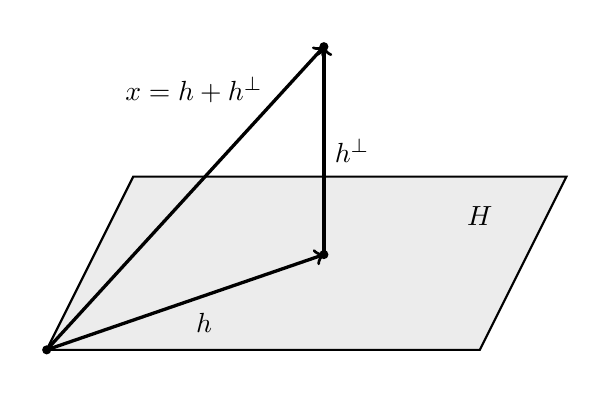
\begin{tikzpicture}[scale=1.1]

    % координаты
    \coordinate (O) at (0,0);
    \coordinate (A) at (5,0);
    \coordinate (B) at (6,2);
    \coordinate (C) at (1,2);

    \coordinate (H) at (3.2,1.1);
    \coordinate (X) at (3.2,3.5);

    % плоскость H
    \filldraw[fill=gray!15, draw=black, thick]
        (O) -- (A) -- (B) -- (C) -- cycle;

    \node at (5.0,1.55) {$H$};

    % оси/направления на плоскости
    

    % проекция h
    \draw[->, very thick] (O) -- (H) node[midway, below right] {$h$};

    % ортогональная составляющая
    \draw[->, very thick] (H) -- (X) node[midway, right] {$h^{\perp}$};

    % исходный вектор x
    \draw[->, very thick] (O) -- (X) node[midway, left] {};

    % пунктир от x к проекции
    \draw[dashed] (X) -- (H);


    % точки
    \fill (O) circle (1.5pt) node[below left] {};
    \fill (H) circle (1.5pt) node[below] {};
    \fill (X) circle (1.5pt) node[above] {};

    % подпись разложения
    \node at (1.7,3.0) {$x = h + h^{\perp}$};

\end{tikzpicture}
\end{center}

\subsection{Выпишите формулу для ортогональной проекции вектора на подпространство, заданное как линейная оболочка данного линейно независимого набора векторов.}

\subsection{Дайте определение линейного многообразия и опишите его связь с линейным подпространством.}

\subsection{Выпишите формулу для вычисления расстояния до многообразия через ортогональную составляющую.}

\subsection{Выпишите формулу для вычисления расстояния до многообразия с помощью определителей матриц Грама.}

\subsection{Дайте определение сопряженного оператора в евклидовом пространстве.}

\subsection{Дайте определение самосопряженного (симметрического) оператора.}

\subsection{Как найти матрицу сопряженного оператора в произвольном базисе?}

\subsection{Каким свойством обладают собственные значения самосопряженного оператора?}

\subsection{Что можно сказать про собственные векторы самосопряженного оператора, отвечающие разным собственным значениям?}

\subsection{Сформулируйте теорему о существовании для самосопряженного оператора базиса из собственных векторов.}

\subsection{Сформулируйте определение ортогональной матрицы.}

\subsection{Сформулируйте определение ортогонального оператора.}

\subsection{Сформулируйте критерий ортогональности оператора, использующий ортонормированный базис.}

\subsection{Сформулируйте критерий ортогональности оператора, использующий его матрицу.}

\subsection{Каков канонический вид ортогонального оператора? Сформулируйте теорему Эйлера.}

\subsection{Сформулируйте теорему о спектральном разложении симметрической матрицы.}

\subsection{Сформулируйте теорему о приведении квадратичной формы к диагональному виду при помощи ортогональной замены координат.}

\subsection{Сформулируйте утверждение о QR-разложении.}

\subsection{Сформулируйте теорему о сингулярном разложении.}

\subsection{Сформулируйте утверждение о полярном разложении.}

\begin{center}
    {\Huge \textbf{Доказательства}}
\end{center}
\addcontentsline{toc}{section}{Доказательства}

\section{Модуль}

\subsection{Докажите, что характеристика поля может быть либо простым числом, либо нулем.}

\begin{theorem}
    \[
        \operatorname{char} P =
        \begin{cases}
            0, \\
            p,\ p \text{ --- простое}
        \end{cases}
    \]
\end{theorem}

\begin{Proof}
    Пусть $p \neq 0 \Rightarrow p \geq 2$.
    
    \[
        p \neq 1,\ \text{т.к. } 1 \neq 0
    \]
    
    Предположим, что $p$ --- не простое. Тогда
    \[
        p = mk,
    \]
    где
    \[
        1 < m,\ k < p.
    \]
    
    По определению характеристики поля:
    \[
        \underbrace{1 + \ldots + 1}_{p} = 0.
    \]
    
    Тогда
    \[
        0
        =
        \underbrace{1 + \ldots + 1}_{mk}
        =
        (\underbrace{1 + \ldots + 1}_{m})
        (\underbrace{1 + \ldots + 1}_{k}).
    \]
    
    Обе скобки не равны нулю, так как $p$ --- минимальное натуральное число, для которого
    \[
        \underbrace{1 + \ldots + 1}_{p} = 0,
    \]
    а
    \[
        m < p,\quad k < p.
    \]
    
    Получили произведение двух ненулевых элементов поля, равное нулю:
    \[
        (\underbrace{1 + \ldots + 1}_{m})
        (\underbrace{1 + \ldots + 1}_{k}) = 0.
    \]
    
    Значит, $m$ и $k$ --- делители нуля, а их нет в поле по определению.
    
    Получили противоречие.
    
    Следовательно, если $\operatorname{char} P \neq 0$, то
    \[
        \operatorname{char} P = p,
    \]
    где $p$ --- простое число.
\end{Proof}

\subsection{Сформулируйте и докажите утверждение о том, каким будет простое подполе в зависимости от характеристики.}

\begin{theorem}
    Пусть $P$ --- поле, а $P_0$ --- его простое подполе. Тогда:
    \[
        1)\ \text{если } \operatorname{char} P = p > 0,\ \text{то } P_0 \cong \mathbb{Z}_p
    \]
    \[
        2)\ \text{если } \operatorname{char} P = 0,\ \text{то } P_0 \cong \mathbb{Q}
    \]
\end{theorem}

\begin{Proof}
    Рассмотрим $1 \in P$ --- нейтральный элемент по умножению.
    
    Тогда
    \[
        \langle 1 \rangle \subset (P,+),
    \]
    где $\langle 1 \rangle$ --- циклическая группа по сложению, порождённая $1$.
    
    Кольцо $\langle 1 \rangle$ является подкольцом в $P$.
    
    Так как любое подполе поля $P$ содержит $1$, то оно содержит и $\langle 1 \rangle$, т.е.
    \[
        \langle 1 \rangle \subset P_0.
    \]
    
    \bigskip
    
    1) Если
    \[
        \operatorname{char} P = p > 0,
    \]
    то
    \[
        \langle 1 \rangle \cong \mathbb{Z}_p.
    \]
    Так как $\mathbb{Z}_p$ --- поле, то
    \[
        P_0 = \langle 1 \rangle \cong \mathbb{Z}_p.
    \]
    
    \bigskip
    
    2) Если
    \[
        \operatorname{char} P = 0,
    \]
    то
    \[
        \langle 1 \rangle \cong \mathbb{Z}.
    \]
    Но $\mathbb{Z}$ --- не поле, значит, в $P_0$ должны быть все дроби вида
    \[
        \frac{a}{b},
    \]
    где
    \[
        a,b \in \langle 1 \rangle,\quad b \neq 0.
    \]
    
    Эти дроби образуют подполе, изоморфное $\mathbb{Q}$.
    
    Следовательно,
    \[
        P_0 \cong \mathbb{Q}.
    \]
\end{Proof}

\subsection{Сформулируйте и докажите критерий того, что кольцо вычетов по модулю $n$ является полем.}

\begin{theorem}
    \[
        \mathbb{Z}_n \text{ является полем } \Longleftrightarrow n \text{ --- простое.}
    \]
\end{theorem}

\begin{Proof}
    Для любого $n$ кольцо $\mathbb{Z}_n$ является кольцом с $1$.

    \bigskip

    {\bf $(\Rightarrow):$}

    Пусть $\mathbb{Z}_n$ --- поле.

    Предположим, что $n$ является составным, тогда
    \[
        n = mk,
    \]
    где
    \[
        1 < m,k < n.
    \]

    Тогда в $\mathbb{Z}_n$:
    \[
        \overline{m}\cdot \overline{k}
        =
        \overline{mk}
        =
        \overline{n}
        =
        \overline{0}.
    \]

    При этом
    \[
        \overline{m}\neq \overline{0},
        \qquad
        \overline{k}\neq \overline{0}.
    \]

    Значит, в $\mathbb{Z}_n$ есть делители нуля, следовательно, это не поле.

    Получили противоречие. Значит, $n$ --- простое.

    \bigskip

    {\bf $(\Leftarrow):$}

    Пусть $n = p$ --- простое.

    Рассмотрим
    \[
        \mathbb{Z}_p =
        \{\overline{0},\overline{1},\ldots,\overline{p-1}\}.
    \]

    Нужно показать, что любой ненулевой элемент обратим.

    Возьмём произвольный
    \[
        \overline{s}\in \mathbb{Z}_p,\qquad \overline{s}\neq \overline{0}.
    \]

    Рассмотрим множество
    \[
        A =
        \{\overline{s}\cdot\overline{1},
        \overline{s}\cdot\overline{2},
        \ldots,
        \overline{s}\cdot\overline{p-1}\}.
    \]

    Покажем, что в $A$ нет $\overline{0}$.

    Если
    \[
        \overline{s}\cdot\overline{k}=\overline{0},
    \]
    то
    \[
        p\mid sk.
    \]
    Так как $p$ --- простое и $p\nmid s$, то
    \[
        p\mid k.
    \]
    Но
    \[
        k\in\{1,\ldots,p-1\},
    \]
    значит, это невозможно.

    Теперь покажем, что элементы множества $A$ попарно различны.

    Пусть
    \[
        \overline{s}\cdot\overline{k_1}
        =
        \overline{s}\cdot\overline{k_2}.
    \]
    Тогда
    \[
        \overline{s}\cdot(\overline{k_1}-\overline{k_2})
        =
        \overline{0}.
    \]
    Отсюда
    \[
        p\mid s(k_1-k_2).
    \]
    Так как $p\nmid s$, то
    \[
        p\mid (k_1-k_2).
    \]
    Но
    \[
        k_1,k_2\in\{1,\ldots,p-1\},
    \]
    поэтому возможно только
    \[
        k_1=k_2.
    \]

    Значит, в $A$ стоят те же элементы, что и в
    \[
        \{\overline{1},\overline{2},\ldots,\overline{p-1}\},
    \]
    только в другом порядке.

    Следовательно, среди элементов $A$ найдётся $\overline{1}$, то есть
    \[
        \exists \overline{t}\in \mathbb{Z}_p:
        \quad
        \overline{s}\cdot\overline{t}
        =
        \overline{1}.
    \]

    Значит, произвольный ненулевой элемент $\overline{s}$ обратим.

    Следовательно,
    \[
        \mathbb{Z}_p \text{ --- поле.}
    \]
\end{Proof}

\subsection{Докажите, что ядро гомоморфизма колец является идеалом.}
\begin{lemma}
    $\operatorname{Ker}\varphi$, где $\varphi$ --- гомоморфизм колец, всегда является идеалом в кольце $K_1$:
    \[
        \varphi: K_1 \to K_2.
    \]
\end{lemma}

\begin{Proof}
    Идеал:
    \[
        1)\ \text{подгруппа в } (K_1,+)
    \]
    \[
        2)\ \forall a \in \operatorname{Ker}\varphi\ \forall r \in K_1:
        \quad ar \in \operatorname{Ker}\varphi
        \text{ и }
        ra \in \operatorname{Ker}\varphi.
    \]

    Так как гомоморфизм колец является гомоморфизмом их аддитивных групп
    $(K_1,+)$ и $(K_2,+)$, то
    \[
        \operatorname{Ker}\varphi
    \]
    является нормальной подгруппой в $(K_1,+)$.
    
    Значит, первое условие идеала выполнено.

    Пусть
    \[
        a \in \operatorname{Ker}\varphi,
    \]
    т.е.
    \[
        \varphi(a)=0.
    \]

    Возьмём произвольный
    \[
        r \in K_1.
    \]

    Рассмотрим:
    \[
        \varphi(ar)
        =
        \varphi(a)\cdot \varphi(r)
        =
        0\cdot \varphi(r)
        =
        0.
    \]
    Значит,
    \[
        ar \in \operatorname{Ker}\varphi.
    \]

    Аналогично:
    \[
        \varphi(ra)
        =
        \varphi(r)\cdot \varphi(a)
        =
        \varphi(r)\cdot 0
        =
        0.
    \]
    Значит,
    \[
        ra \in \operatorname{Ker}\varphi.
    \]

    Следовательно,
    \[
        \operatorname{Ker}\varphi
    \]
    является идеалом в $K_1$.
\end{Proof}

\subsection{Сформулируйте и докажите теорему о гомоморфизме колец.}

\begin{theorem}[О гомоморфизме колец]
    Пусть $K_1, K_2$ --- два кольца,
    \[
        \varphi: K_1 \to K_2
    \]
    --- гомоморфизм. Тогда
    \[
        K_1 / \operatorname{Ker}\varphi \cong \operatorname{Im}\varphi.
    \]
\end{theorem}

\begin{Proof}
    Ядро $\operatorname{Ker}\varphi$ является идеалом, поэтому
    \[
        K_1 / \operatorname{Ker}\varphi
    \]
    корректно определено.

    Рассмотрим отображение
    \[
        \tau: K_1 / \operatorname{Ker}\varphi \to \operatorname{Im}\varphi
    \]
    по правилу
    \[
        \tau(a + \operatorname{Ker}\varphi) = \varphi(a).
    \]

    Из теоремы о гомоморфизме групп следует, что $\tau$ корректно определено и является гомоморфизмом групп по сложению.

    Остаётся проверить, что $\tau$ сохраняет умножение:
    \[
        \tau((a + \operatorname{Ker}\varphi)(b + \operatorname{Ker}\varphi))
        =
        \tau(ab + \operatorname{Ker}\varphi)
    \]
    \[
        =
        \varphi(ab)
        =
        \varphi(a)\varphi(b)
        =
        \tau(a + \operatorname{Ker}\varphi)\tau(b + \operatorname{Ker}\varphi).
    \]

    Значит, $\tau$ --- гомоморфизм колец.

    Так как $\tau$ является биекцией из теоремы о гомоморфизме групп, то
    \[
        K_1 / \operatorname{Ker}\varphi \cong \operatorname{Im}\varphi.
    \]
\end{Proof}

\subsection{Сформулируйте и докажите утверждение о том, когда факторкольцо кольца многочленов над полем само является полем.}
\begin{theorem}
    Пусть $P$ --- поле, а $f(x) \in P[x]$. Тогда факторкольцо
    \[
        P[x]/\langle f(x) \rangle
    \]
    является полем
    \[
        \Longleftrightarrow
    \]
    многочлен $f(x)$ неприводим над $P$.
\end{theorem}

\begin{Proof}
    {\bf $(\Rightarrow):$}

    Пусть
    \[
        P[x]/\langle f(x) \rangle
    \]
    --- поле.

    Предположим, что $f(x)$ приводим. Тогда
    \[
        f(x)=f_1(x)\cdot f_2(x),
    \]
    где
    \[
        0 < \deg f_1 < \deg f,\qquad 0 < \deg f_2 < \deg f.
    \]

    Рассмотрим классы
    \[
        \overline{f_1},\ \overline{f_2} \in P[x]/\langle f(x) \rangle.
    \]

    Они отличны от нуля, так как
    \[
        \deg f_1 < \deg f,\qquad \deg f_2 < \deg f.
    \]

    Но
    \[
        \overline{f_1}\cdot \overline{f_2}
        =
        \overline{f_1f_2}
        =
        \overline{f}
        =
        \overline{0}.
    \]

    Значит, в факторкольце есть делители нуля, следовательно, оно не поле.

    Получили противоречие. Значит, $f(x)$ неприводим над $P$.

    \bigskip

    {\bf $(\Leftarrow):$}

    Пусть $f(x)$ неприводим над $P$.

    Покажем, что любой ненулевой класс
    \[
        \overline{a(x)} \neq \overline{0}
    \]
    обратим в
    \[
        P[x]/\langle f(x) \rangle.
    \]

    Возьмём представителя $a(x)$ такой, что
    \[
        \deg a(x) < \deg f(x).
    \]

    Так как
    \[
        \overline{a(x)} \neq \overline{0},
    \]
    то $a(x)$ не делится на $f(x)$.

    Поскольку $f(x)$ неприводим, то
    \[
        \gcd(a(x), f(x)) = 1.
    \]

    Значит, существуют многочлены $b(x), c(x) \in P[x]$ такие, что
    \[
        a(x)b(x) + c(x)f(x) = 1.
    \]

    Переходя к классам по модулю $\langle f(x) \rangle$, получаем:
    \[
        \overline{a}\cdot \overline{b} + \overline{c}\cdot \overline{f}
        =
        \overline{1}.
    \]

    Так как
    \[
        \overline{f} = \overline{0},
    \]
    то
    \[
        \overline{a}\cdot \overline{b} = \overline{1}.
    \]

    Значит, $\overline{b}$ --- обратный элемент к $\overline{a}$ в
    \[
        P[x]/\langle f(x) \rangle.
    \]

    Следовательно, каждый ненулевой элемент факторкольца обратим, значит
    \[
        P[x]/\langle f(x) \rangle
    \]
    является полем.
\end{Proof}
\subsection{Выпишите и докажите формулу для описания изменения координат вектора при изменении базиса.}

\begin{theorem}
    Пусть $x \in L$, $\mathcal{A}$ и $\mathcal{B}$ --- базисы в $L$.
    
    \[
        x^a = (x_1^a, \ldots, x_n^a)^T
    \]
    --- столбец координат вектора $x$ в базисе $\mathcal{A}$.
    
    \[
        x^b = (x_1^b, \ldots, x_n^b)^T
    \]
    --- столбец координат вектора $x$ в базисе $\mathcal{B}$.
    
    Тогда
    \[
        x^b = T_{\mathcal{A} \to \mathcal{B}}^{-1}x^a
        \Longleftrightarrow
        X' = T^{-1}X,
    \]
    где $X'$ --- координаты в новом базисе.
\end{theorem}

\begin{Proof}
    Докажем, что
    \[
        x^b = T_{\mathcal{A} \to \mathcal{B}}^{-1}x^a.
    \]
    
    Пусть
    \[
        \mathcal{A} = (a_1, \ldots, a_n),
        \qquad
        \mathcal{B} = (b_1, \ldots, b_n).
    \]
    
    Тогда
    \[
        x
        =
        \mathcal{A}x^a
        =
        (a_1, \ldots, a_n)
        \begin{pmatrix}
            x_1^a \\
            \vdots \\
            x_n^a
        \end{pmatrix}
        =
        x_1^a a_1 + \ldots + x_n^a a_n
        =
        \mathcal{B}x^b.
    \]
    
    По определению матрицы перехода:
    \[
        \mathcal{B}
        =
        \mathcal{A}T_{\mathcal{A} \to \mathcal{B}}.
    \]
    
    Поэтому
    \[
        \mathcal{A}x^a
        =
        \mathcal{B}x^b
        =
        \mathcal{A}T_{\mathcal{A} \to \mathcal{B}}x^b.
    \]
    
    Так как $\mathcal{A}$ --- базис, получаем:
    \[
        x^a
        =
        T_{\mathcal{A} \to \mathcal{B}}x^b.
    \]
    
    Следовательно,
    \[
        x^b
        =
        T_{\mathcal{A} \to \mathcal{B}}^{-1}x^a.
    \]
\end{Proof}

\subsection{Сформулируйте и докажите утверждение о связи размерности суммы и пересечения подпространств.}
\begin{theorem}
    Пусть $H_1$ и $H_2$ --- подпространства в $L$. Тогда:
    \[
        \dim(H_1 + H_2)
        =
        \dim(H_1) + \dim(H_2) - \dim(H_1 \cap H_2)
    \]
\end{theorem}

\begin{Proof}
    Рассмотрим базис $H_1 \cap H_2$. Дополним его до базиса в $H_1$ и до базиса в $H_2$.
    
    Пусть
    \[
        \dim H_1 = n,\quad \dim H_2 = m,\quad \dim(H_1 \cap H_2) = r.
    \]
    
    Обозначим базисные векторы следующим образом:
    \[
        \underbrace{e_1,\ldots,e_r}_{\text{базис в } H_1 \cap H_2},
        \quad
        \underbrace{v_1,\ldots,v_{n-r}}_{\text{дополнение до } H_1},
        \quad
        \underbrace{w_1,\ldots,w_{m-r}}_{\text{дополнение до } H_2}.
    \]
    
    Это базис в $H_1 + H_2$, т.к. любой вектор из $H_1 + H_2$ может быть выражен через них, и они л.н.з.
    
    Таким образом, можем найти размерность $H_1 + H_2$:
    \[
        \dim(H_1 + H_2)
        =
        r + (n-r) + (m-r)
        =
        n + m - r
    \]
    \[
        =
        \dim H_1 + \dim H_2 - \dim(H_1 \cap H_2).
    \]
\end{Proof}
\subsection{Что такое сумма и прямая сумма подпространств? Сформулируйте и докажите критерий того, что сумма подпространств является прямой.}
\begin{definition}
    Множество
    \[
        H_1 + H_2 =
        \{x_1 + x_2\ |\ x_1 \in H_1,\ x_2 \in H_2\}
    \]
    называется суммой подпространств $H_1$ и $H_2$.
\end{definition}

\begin{definition}
    Сумма подпространств $H_1 + H_2$ называется прямой и обозначается
    \[
        H_1 \oplus H_2,
    \]
    где
    \[
        H_1 \cap H_2 = \{0\},
    \]
    т.е. тривиально.
\end{definition}

\begin{theorem}
    \[
        H_1 + H_2 \text{ является прямой суммой}
    \]
    \[
        \Longleftrightarrow
    \]
    $\forall x \in H_1 + H_2$ единственным образом представляется в виде
    \[
        x = x_1 + x_2,
    \]
    где
    \[
        x_1 \in H_1,\quad x_2 \in H_2.
    \]
\end{theorem}

\begin{Proof}
    {\bf Необходимость.}

    Дано: сумма прямая, т.е.
    \[
        H_1 \cap H_2 = \{0\}.
    \]
    Докажем, что
    \[
        x = x_1 + x_2
    \]
    представляется единственным образом.

    Предположим, что есть два разложения:
    \[
        x = x_1 + x_2
    \]
    и
    \[
        x = y_1 + y_2,
    \]
    где
    \[
        x_1,y_1 \in H_1,\quad x_2,y_2 \in H_2.
    \]

    Вычтем их друг из друга:
    \[
        x_1 + x_2 = y_1 + y_2
    \]
    \[
        x_1 - y_1 = y_2 - x_2.
    \]

    Так как
    \[
        x_1 - y_1 \in H_1,
    \]
    и
    \[
        y_2 - x_2 \in H_2,
    \]
    то
    \[
        x_1 - y_1 = y_2 - x_2 \in H_1 \cap H_2.
    \]

    Но
    \[
        H_1 \cap H_2 = \{0\},
    \]
    значит
    \[
        x_1 - y_1 = y_2 - x_2 = 0.
    \]

    Следовательно,
    \[
        x_1 = y_1,\quad x_2 = y_2.
    \]

    Значит, представление единственно.

    \bigskip

    {\bf Достаточность.}

    Дано: каждый
    \[
        x \in H_1 + H_2
    \]
    представляется единственным образом в виде
    \[
        x = x_1 + x_2.
    \]

    Докажем, что сумма прямая, т.е.
    \[
        H_1 \cap H_2 = \{0\}.
    \]

    Предположим противное:
    \[
        \exists x \neq 0:\quad x \in H_1 \cap H_2.
    \]

    Тогда
    \[
        x \in H_1
        \quad \text{и} \quad
        x \in H_2.
    \]

    Для любого $\beta \in F$ имеем:
    \[
        x = x - \beta x + \beta x
        =
        (1-\beta)x + \beta x.
    \]

    Причём
    \[
        (1-\beta)x \in H_1,
        \qquad
        \beta x \in H_2.
    \]

    Значит, у $x$ есть разные представления в виде суммы элемента из $H_1$ и элемента из $H_2$.

    Получили противоречие с единственностью представления.

    Следовательно,
    \[
        H_1 \cap H_2 = \{0\}.
    \]

    Значит,
    \[
        H_1 + H_2 = H_1 \oplus H_2.
    \]
\end{Proof}

\section{Модуль}

\subsection{Выпишите формулу для преобразования матрицы билинейной формы при замене базиса и докажите её.}
\begin{theorem}
    Пусть $U$ --- матрица перехода от базиса $e$ к базису $f$.
    
    Пусть $B_e$ --- матрица билинейной формы в базисе $e$.
    
    Тогда
    \[
        B_f = U^T B_e U.
    \]
\end{theorem}

\begin{Proof}
    Пусть
    \[
        b(x,y)
    \]
    --- билинейная форма.
    
    В базисе $e$ она записывается так:
    \[
        b(x,y) = x_e^T B_e y_e,
    \]
    где $x_e,\ y_e$ --- столбцы координат векторов $x$ и $y$ в базисе $e$.
    
    Так как $U$ --- матрица перехода от базиса $e$ к базису $f$, то
    \[
        x_e = Ux_f,
        \qquad
        y_e = Uy_f,
    \]
    где $x_f,\ y_f$ --- столбцы координат векторов $x$ и $y$ в базисе $f$.
    
    Подставим это в формулу билинейной формы:
    \[
        b(x,y)
        =
        (Ux_f)^T B_e (Uy_f).
    \]
    
    Тогда
    \[
        b(x,y)
        =
        x_f^T U^T B_e U y_f.
    \]
    
    С другой стороны, в базисе $f$:
    \[
        b(x,y) = x_f^T B_f y_f.
    \]
    
    Значит,
    \[
        x_f^T B_f y_f
        =
        x_f^T U^T B_e U y_f.
    \]
    
    Следовательно,
    \[
        B_f = U^T B_e U.
    \]
\end{Proof}

\subsection{Сформулируйте и докажите \textnormal{(включая лемму)} теорему об инвариантности ранга матрицы квадратичной формы.}

\begin{lemma}
    Пусть
    \[
        A,S \in M_n(\mathbb{R}),
        \qquad
        \det S \neq 0.
    \]
    Тогда
    \[
        Rg(A\cdot S) = Rg(A) = Rg(S\cdot A),
    \]
    то есть умножение на невырожденную матрицу $S$ не меняет ранг матрицы $A$.
\end{lemma}

\begin{Proof}
    Докажем, что
    \[
        Rg(A\cdot S) = Rg(A).
    \]
    
    Сначала
    \[
        Rg(A\cdot S) \leq Rg(A),
    \]
    так как столбцы матрицы $A\cdot S$ --- это линейные комбинации столбцов матрицы $A$, а ранг равен максимальному количеству л.н.з. столбцов.
    
    С другой стороны, так как $\det S \neq 0$, то существует $S^{-1}$. Поэтому
    \[
        A = A\cdot S \cdot S^{-1}.
    \]
    Тогда аналогично
    \[
        Rg(A) = Rg(A\cdot S\cdot S^{-1}) \leq Rg(A\cdot S).
    \]
    
    Следовательно,
    \[
        Rg(A\cdot S)=Rg(A).
    \]
    
    Аналогично доказывается, что
    \[
        Rg(S\cdot A)=Rg(A).
    \]
\end{Proof}

\begin{theorem}[Об инвариантности ранга]
    Пусть $Q$ --- квадратичная форма на линейном пространстве $V$,
    \[
        a = a_1,\ldots,a_n,
        \qquad
        b = b_1,\ldots,b_n
    \]
    --- базисы в $V$.
    
    Пусть $A$ --- матрица $Q(x)$ в базисе $a$, а $B$ --- матрица $Q(x)$ в базисе $b$.
    
    Тогда
    \[
        RgA = RgB.
    \]
\end{theorem}

\begin{Proof}
    Мы знаем, что при замене базиса матрица квадратичной формы преобразуется по формуле
    \[
        B = S^TAS,
    \]
    где
    \[
        S = T_{a \to b}
    \]
    --- матрица перехода, и она всегда невырожденная.
    
    По лемме при умножении $A$ на невырожденные матрицы $S$ и $S^T$ её ранг не изменяется.
    
    Значит,
    \[
        RgB = Rg(S^TAS) = RgA.
    \]
\end{Proof}


\subsection{Сформулируйте и докажите утверждение о том, что действие линейного оператора полностью задаётся его матрицей.}

\begin{theorem}
    Пусть $\varphi(x): V \to V$ --- линейный оператор в л.п. $V$.
    
    Пусть $e_1,\ldots,e_n$ --- базис в $V$, рассмотрим вектор
    \[
        x \in V
    \]
    и
    \[
        x^e =
        \begin{pmatrix}
            x_1 \\
            \vdots \\
            x_n
        \end{pmatrix}
    \]
    --- столбец координат вектора $x$ в базисе $e_1,\ldots,e_n$.
    
    Тогда
    \[
        (\varphi(x))^e = A_e x^e.
    \]
\end{theorem}

\begin{Proof}
    Так как $e_1,\ldots,e_n$ --- базис в $V$, то
    \[
        x = x_1e_1 + \ldots + x_ne_n.
    \]
    
    Тогда по линейности оператора:
    \[
        \varphi(x)
        =
        \varphi(x_1e_1 + \ldots + x_ne_n)
    \]
    \[
        =
        x_1\varphi(e_1) + \ldots + x_n\varphi(e_n).
    \]
    
    Разложим образы базисных векторов по базису $e_1,\ldots,e_n$:
    \[
        \varphi(e_1) = a_{11}e_1 + \ldots + a_{n1}e_n,
    \]
    \[
        \ldots
    \]
    \[
        \varphi(e_n) = a_{1n}e_1 + \ldots + a_{nn}e_n.
    \]
    
    Подставим:
    \[
        \varphi(x)
        =
        x_1(a_{11}e_1 + \ldots + a_{n1}e_n)
        + \ldots +
        x_n(a_{1n}e_1 + \ldots + a_{nn}e_n).
    \]
    
    Соберём коэффициенты при $e_1,\ldots,e_n$:
    \[
        \varphi(x)
        =
        (a_{11}x_1 + \ldots + a_{1n}x_n)e_1
        + \ldots +
        (a_{n1}x_1 + \ldots + a_{nn}x_n)e_n.
    \]
    
    Значит,
    \[
        (\varphi(x))^e
        =
        \begin{pmatrix}
            a_{11}x_1 + \ldots + a_{1n}x_n \\
            \vdots \\
            a_{n1}x_1 + \ldots + a_{nn}x_n
        \end{pmatrix}
        =
        A_e
        \begin{pmatrix}
            x_1 \\
            \vdots \\
            x_n
        \end{pmatrix}.
    \]
    
    Следовательно,
    \[
        (\varphi(x))^e = A_e x^e.
    \]
\end{Proof}
\subsection{Выпишите формулу для преобразования матрицы линейного отображения и матрицы линейного оператора при замене базиса и докажите её в случае линейного оператора.}

\subsection{Сформулируйте и докажите утверждение о связи размерностей ядра и образа линейного отображения.}
\begin{theorem}
    Пусть
    \[
        \varphi: V_1 \to V_2
    \]
    --- линейное отображение. Тогда
    \[
        \dim \operatorname{Ker}\varphi + \dim \operatorname{Im}\varphi
        =
        \dim V_1.
    \]
\end{theorem}

\begin{Proof}
    Выберем базис в $V_1$:
    \[
        e = e_1,\ldots,e_m.
    \]
    
    Тогда любой $x \in V_1$ можно представить в виде:
    \[
        x = x_1e_1 + \ldots + x_me_m.
    \]
    
    Следовательно,
    \[
        \varphi(x)
        =
        x_1\varphi(e_1) + \ldots + x_m\varphi(e_m),
    \]
    где
    \[
        \varphi(e_1),\ldots,\varphi(e_m)
    \]
    --- столбцы матрицы линейного отображения $\varphi$.
    
    Тогда
    \[
        \operatorname{Im}\varphi
        =
        L(\varphi(e_1),\ldots,\varphi(e_m)).
    \]
    
    Значит,
    \[
        \dim \operatorname{Im}\varphi = RgA,
    \]
    где $A$ --- матрица линейного отображения $\varphi$.
    
    Ядро отображения записывается однородной системой:
    \[
        Ax = 0.
    \]
    
    Поэтому
    \[
        \dim \operatorname{Ker}\varphi
    \]
    --- это число элементов ФСР системы
    \[
        Ax = 0.
    \]
    
    По теореме о ФСР:
    \[
        \dim \operatorname{Ker}\varphi = m - RgA.
    \]
    
    Тогда
    \[
        \dim \operatorname{Ker}\varphi + \dim \operatorname{Im}\varphi
        =
        (m - RgA) + RgA
        =
        m
        =
        \dim V_1.
    \]
\end{Proof}
\subsection{Сформулируйте и докажите утверждение о связи характеристического уравнения и спектра линейного оператора.}

\begin{theorem}
    $\lambda$ --- собственное значение линейного оператора $A$
    \[
        \Longleftrightarrow
    \]
    $\lambda$ --- корень характеристического многочлена
    
    над алгебраически замкнутым полем или, если корень принадлежит рассматриваемому полю $F$.
\end{theorem}

\begin{Proof}
    {\bf Необходимость.}
    
    Дано:
    \[
        \lambda \text{ --- собственное значение}
    \]
    
    Докажем:
    \[
        \lambda \text{ --- корень характеристического многочлена.}
    \]
    
    По определению
    \[
        \exists x \neq 0:\quad Ax = \lambda x.
    \]
    
    Тогда
    \[
        Ax = \lambda I x
        \Longleftrightarrow
        (A-\lambda I)x = 0,
    \]
    где $I$ --- единичная матрица.
    
    Запишем равенство $(A-\lambda I)x=0$ в некотором базисе $e$:
    \[
        (A_e-\lambda E)x^e = 0.
    \]
    
    Это однородная СЛАУ, и она имеет ненулевое решение, $x$ --- собственный (ненулевой) вектор.
    
    Значит,
    \[
        \det(A_e-\lambda E)=0.
    \]
    
    Следовательно, $\lambda$ --- корень характеристического уравнения.
    
    \bigskip
    
    {\bf Достаточность.}
    
    Дано:
    \[
        \lambda \text{ --- корень характеристического многочлена.}
    \]
    
    Докажем:
    \[
        \lambda \text{ --- с.з.}
    \]
    
    Если $\lambda$ --- корень, то в заданном базисе:
    \[
        \det(A_e-\lambda E)=0.
    \]
    
    Значит, однородная СЛАУ
    \[
        (A_e-\lambda E)x^e=0
    \]
    имеет ненулевое решение.
    
    Это решение можно интерпретировать как набор координат некоторого ненулевого вектора $x$, для которого
    \[
        (A-\lambda I)x=0.
    \]
    
    Тогда
    \[
        Ax=\lambda x,\qquad x\neq 0.
    \]
    
    Следовательно, $x$ --- с.в., а $\lambda$ --- с.з.
\end{Proof}

\subsection{Сформулируйте и докажите утверждение о том, каким свойством обладают собственные векторы линейного оператора, отвечающие различным собственным значениям.}

\begin{theorem}
    Пусть $\lambda_1, \ldots, \lambda_k$ --- с.з. линейного оператора $A$,
    \[
        \lambda_i \neq \lambda_j,\quad i \neq j,
    \]
    а $v_1,\ldots,v_k$ --- соответствующие с.в.
    
    Тогда
    \[
        v_1,\ldots,v_k
    \]
    --- линейно независимые.
    
    То есть с.в., отвечающие различным с.з., линейно независимы.
\end{theorem}

\begin{Proof}
    Применим принцип математической индукции.
    
    При $k = 1$ верно, так как с.в. по определению не $0$ и, соответственно, л.н.з.
    
    Пусть утверждение верно для $k = m$.
    
    Добавим ещё один с.в. $v_{m+1}$. Докажем, что система из векторов
    \[
        v_1,\ldots,v_m,v_{m+1}
    \]
    осталась л.н.з.
    
    Рассмотрим равенство:
    \[
        \alpha_1v_1+\alpha_2v_2+\ldots+\alpha_mv_m+\alpha_{m+1}v_{m+1}=0.
    \]
    
    Применим к нему линейный оператор $A$:
    \[
        \alpha_1\lambda_1v_1+\ldots+\alpha_m\lambda_mv_m
        +\alpha_{m+1}\lambda_{m+1}v_{m+1}=0.
    \]
    
    Умножим первое равенство на $\lambda_{m+1}$:
    \[
        \alpha_1\lambda_{m+1}v_1+\ldots+\alpha_m\lambda_{m+1}v_m
        +\alpha_{m+1}\lambda_{m+1}v_{m+1}=0.
    \]
    
    Вычтем это равенство из предыдущего:
    \[
        \alpha_1(\lambda_1-\lambda_{m+1})v_1
        +\ldots+
        \alpha_m(\lambda_m-\lambda_{m+1})v_m
        =
        0.
    \]
    
    Так как $\lambda_i$ различны, а
    \[
        v_1,\ldots,v_m
    \]
    --- л.н.з. по предположению индукции, то
    \[
        \alpha_1(\lambda_1-\lambda_{m+1})=0,
        \ldots,
        \alpha_m(\lambda_m-\lambda_{m+1})=0.
    \]
    
    Значит
    \[
        \alpha_1=\ldots=\alpha_m=0.
    \]
    
    Тогда исходное равенство принимает вид:
    \[
        \alpha_{m+1}v_{m+1}=0.
    \]
    
    Так как $v_{m+1}$ --- с.в., то
    \[
        v_{m+1}\neq 0.
    \]
    
    Следовательно,
    \[
        \alpha_{m+1}=0.
    \]
    
    Значит,
    \[
        v_1,\ldots,v_m,v_{m+1}
    \]
    --- л.н.з.
    
    Шаг выполнен, значит утверждение верно всегда.
\end{Proof}
\subsection{Сформулируйте и докажите критерий диагональности матрицы оператора.}

\begin{theorem}
    Матрица линейного оператора является диагональной в данном базисе
    \[
        \Longleftrightarrow
    \]
    все векторы этого базиса являются собственными векторами для данного линейного оператора
\end{theorem}

\begin{Proof}
    {\bf Необходимость.}

    Дано:
    \[
        A_e \text{ --- диагональна.}
    \]

    Докажем:
    \[
        \text{базис } e \text{ состоит из собственных векторов.}
    \]

    По определению матрицы линейного оператора в $j$-ом столбце стоят координаты вектора
    \[
        A(e_j)
    \]
    в базисе $e$.

    Если матрица диагональна, то $j$-й столбец имеет вид
    \[
        \begin{pmatrix}
            0 \\
            \vdots \\
            0 \\
            \lambda_j \\
            0 \\
            \vdots \\
            0
        \end{pmatrix},
    \]
    где $\lambda_j$ стоит на $j$-ом месте.

    То есть
    \[
        A(e_j)
        =
        0\cdot e_1+\ldots+0\cdot e_{j-1}
        +\lambda_j e_j
        +0\cdot e_{j+1}+\ldots+0\cdot e_n.
    \]

    Значит,
    \[
        A(e_j)=\lambda_j e_j.
    \]

    Так как
    \[
        e_j \neq 0
    \]
    потому что это элемент базиса, то $e_j$ --- собственный вектор с собственным значением $\lambda_j$.

    Так это верно для
    \[
        \forall j=\overline{1,n},
    \]
    то все базисные векторы --- собственные, а на диагонали стоят собственные значения

    \bigskip

    {\bf Достаточность.}

    Дано:
    \[
        (e_1,\ldots,e_n)
    \]
    --- базис, и он состоит из собственных векторов

    Докажем:
    \[
        A_e \text{ --- диагональная.}
    \]

    Так как каждый $e_j$ --- собственный вектор, то
    \[
        A(e_j)=\lambda_j e_j.
    \]

    По определению матрицы линейного оператора $j$-й столбец матрицы $A_e$ --- это координаты вектора $A(e_j)$ в базисе $e$.

    Но
    \[
        A(e_j)=\lambda_j e_j,
    \]
    значит $j$-й столбец имеет вид
    \[
        \begin{pmatrix}
            0 \\
            \vdots \\
            0 \\
            \lambda_j \\
            0 \\
            \vdots \\
            0
        \end{pmatrix}.
    \]

    Следовательно, все элементы вне диагонали равны нулю, а на диагонали стоят числа
    \[
        \lambda_1,\ldots,\lambda_n.
    \]

    Значит,
    \[
        A_e
    \]
    --- диагональная.
\end{Proof}
\subsection{Каким свойством обладает оператор в $n$-мерном вещественном пространстве, у характеристического многочлена которого есть $n$ различных действительных корней? Ответ обоснуйте.}

\begin{theorem}[Достаточное условие диагонализируемости]
    Если характеристическое уравнение линейного оператора, действующего в $V$, где
    \[
        \dim V = n,
    \]
    имеет $n$ попарно различных корней, то линейный оператор диагонализируем.
    
    Корни лежат в том же поле, над которым рассматривается $V$.
\end{theorem}

\begin{Proof}
    Если $\lambda \in F$ --- корень характеристического уравнения, то ему можно сопоставить хотя бы $1$ собственный вектор.
    
    Пусть
    \[
        \lambda_1,\ldots,\lambda_n
    \]
    --- различные корни характеристического уравнения.
    
    Выберем соответствующие им собственные векторы:
    \[
        v_1,\ldots,v_n.
    \]
    
    Так как собственные векторы, отвечающие различным собственным значениям, линейно независимы, то
    \[
        v_1,\ldots,v_n
    \]
    --- л.н.з.
    
    Их число равно
    \[
        n = \dim V,
    \]
    значит, они образуют базис в $V$.
    
    Этот базис состоит из собственных векторов, поэтому в нём матрица линейного оператора диагональна.
    
    Следовательно, линейный оператор диагонализируем.
\end{Proof}
\subsection{Выпишите и докажите неравенство Коши--Буняковского. Выпишите и докажите неравенство треугольника.}

\begin{theorem}
    $\forall x,y \in E$ справедливо неравенство:
    \[
        |g(x,y)| \leq \|x\|\|y\|.
    \]
\end{theorem}

\begin{Proof}
    \[
        \forall \alpha \in \mathbb{R}\quad
        g(\alpha x-y,\alpha x-y)\geq 0
    \]
    по положительной определённости.

    Раскроем:
    \[
        g(\alpha x-y,\alpha x-y)
        =
        \alpha g(x,\alpha x-y)-g(y,\alpha x-y)
    \]
    \[
        =
        \alpha^2g(x,x)-\alpha g(x,y)-\alpha g(y,x)+g(y,y)
    \]
    \[
        =
        \alpha^2g(x,x)-2\alpha g(x,y)+g(y,y)
    \]
    \[
        =
        \alpha^2\|x\|^2-2\alpha g(x,y)+\|y\|^2 \geq 0,
        \quad \forall \alpha \in \mathbb{R}.
    \]

    Рассмотрим это как квадратный трёхчлен по $\alpha$.
    Так как он неотрицателен при всех $\alpha \in \mathbb{R}$, то его дискриминант
    \[
        D \leq 0.
    \]

    Тогда:
    \[
        D
        =
        4g(x,y)^2-4\|x\|^2\|y\|^2
        \leq 0.
    \]

    Отсюда
    \[
        g(x,y)^2 \leq \|x\|^2\|y\|^2.
    \]

    Следовательно,
    \[
        |g(x,y)| \leq \|x\|\|y\|.
    \]
\end{Proof}

\begin{theorem}[Неравенство треугольника]
    $\forall x,y \in E$
    \[
        \|x+y\| \leq \|x\|+\|y\|.
    \]
\end{theorem}

\begin{Proof}
    \[
        \|x+y\|^2
        =
        g(x+y,x+y)
    \]
    \[
        =
        g(x,x)+2g(x,y)+g(y,y)
    \]
    \[
        \leq
        \|x\|^2+2\|x\|\|y\|+\|y\|^2
    \]
    по неравенству Коши--Буняковского.

    Тогда
    \[
        \|x+y\|^2
        \leq
        (\|x\|+\|y\|)^2.
    \]

    Обе части неотрицательны, следовательно,
    \[
        \|x+y\| \leq \|x\|+\|y\|.
    \]
\end{Proof}
\subsection{Выпишите формулу для преобразования матрицы Грама при переходе к новому базису. Что происходит с определителем матрицы Грама при применении процесса ортогонализации Грама--Шмидта? Что можно сказать про знак определителя матрицы Грама? Всё ответы обоснуйте.}

\subsection{Сформулируйте и докажите критерий линейной зависимости набора векторов с помощью матрицы Грама.}

\subsection{Сформулируйте и докажите теорему о том, как можно представить евклидово пространство с помощью подпространства и его ортогонального дополнения.}

\subsection{Выпишите формулу для ортогональной проекции вектора на подпространство, заданное как линейная оболочка данного линейно независимого набора векторов, и докажите её.}

\subsection{Докажите, что для любого оператора в конечномерном евклидовом пространстве существует единственный сопряженный оператор.}

\subsection{Сформулируйте и докажите свойство собственных векторов самосопряженного оператора, отвечающих разным собственным значениям.}

\subsection{Каким свойством обладают собственные значения самосопряженного оператора? Ответ обоснуйте.}

\subsection{Сформулируйте теорему о существовании для самосопряженного оператора базиса из собственных векторов. Приведите доказательство в случае попарно различных собственных значений.}

\subsection{Сформулируйте и докажите критерий ортогональности оператора, использующий его матрицу.}

\subsection{Сформулируйте и докажите теорему о том, что ортогональный оператор переводит ортонормированный базис в ортонормированный. Верно ли обратно? Ответ обоснуйте.}

\subsection{Сформулируйте и докажите теорему о спектральном разложении симметрической матрицы.}

\subsection{Сформулируйте и докажите утверждение о QR-разложении.}

\subsection{Сформулируйте и докажите теорему о сингулярном разложении.}

\subsection{Сформулируйте и докажите утверждение о полярном разложении.}

\subsection{Сформулируйте и докажите теорему о приведении квадратичных форм к диагональному виду при помощи ортогональной замены координат.}